
%  overview of grading criteria:
%  -----------------------------
%  Structure and readability
%  The structure is clear and easy to follow. Language is clear and precise. 
%  All the key concepts are well introduced. There is a good balance between 
%  comprehension and concision.

%  Executive summary
%  Is informative and covers all the key points of the report thoroughly. It 
%  is standalone and provides a clear picture of the report. Is concise and 
%  to the point. Is engaging and strongly motivates the reader to read the whole 
%  report.

%  Introduction
%  Clear and complete identification of project goals and objectives. The project 
%  and its objectives are well motivated and the background is described clearly. 
%  The length and level of required details are very well balanced.

%  Body
%  Content is comprehensive, accurate, and persuasive. Major points are stated 
%  clearly and are well supported.

%  Evaluation
%  An extensive and clear evaluation of the outcomes of the project with respect 
%  to the project goals and objectives and also compared to previous existing 
%  solutions/systems. The strengths and weaknesses of the outcome and progress 
%  are critically and deeply analyzed

%  Conclusion and suggestions
%  Conclusions are brief, clean-cut and specific, and relate specifically to the 
%  objectives of the project as set out in the introduction. The conclusions follow 
%  logically from the outcomes of the projects. Suggestions are logically connected 
%  to the conclusions, they are action-oriented, feasible, and presented in order of 
%  importance.
 

\documentclass[a4paper,12pt]{article}

% Packages
\usepackage[utf8]{inputenc}
\usepackage{graphicx}    % For including images
\usepackage{amsmath}     % For math
\usepackage{amsfonts}    % For fonts
\usepackage{hyperref}    % For hyperlinks
\usepackage{geometry}    % Page margins
\usepackage{caption}     % Custom captions
\usepackage{float}       % Precise figure placement
\usepackage{natbib}      % Bibliography
\geometry{margin=1in}

% Title and Author
\title{MedAssist: An Automated Solution for The Assessment of Medication Intake}
\author{Adem Kaya, George Lalidis, Giedrius Mirklys, Tam Van}
\date{21-06-2025}
\begin{document}

% Title Page
\maketitle

\section{Introduction}
For the course AI in the Professional Workfield (SOW-MKI76), we were challenged 
to develop a project for a company in a selection of companies provided on the 
Masters Challenge platform. Given our shared background and passion for societal 
impact and healthcare, we ended up with a company called MedAssist.

\subsection{MedAssist}
MedAssist is a company that is concerned with building medication dispensary devices. 
Not only do their devices feature automatic release of medication, such that it 
capable of helping its patients to take their medication on time, but the devices
also feature a build in camera that is capable of recoding videos of the patients 
whenever they are exactly in front of the device. 

\subsection{The Problem}
As of now the video material that is collected by the deviced is manually reviewed by
humans to check whether the patient in question has sucessfully taken their medication. 
The problem lays in the time consuming nature of this process. In order to provide 
a solution to this time consuming approach, MedAssist has reached out to us to 
build an AI which is capable of automatically assessing whether the patient has taken
their medication or not.

\subsection{The Goal}
In order to provide a solution to the problem, the goal is to build an AI which 
is capable of automatically assessing whether the patient has taken their medication
or not to its best extent. Not only should we aim to maximize the accuracy of the
AI, but we should also carefully aim to minimize the amount of false positives as
we do not want the AI to make it seem like the patient has taken their medication 
even though they have not.

\section{Methods}
\subsection{Dataet}
The dataset that was provided to us by MedAssist, initially consisted of 85 unlabeled videos
taken by the medication dispensary devices. We were told beforehand that there were not
privacy concerns applicablel to the dataset, and that we were allowed to use it freely. 
The videos had small variations in lenghts, subjects, surroundings; but did include a 
large variety of different lightning conditions. Each of the 85 videos was watched 
and manually annotated whether the subject took their medication or not. Of these 85 videos,
a total 71 cases where found to contain content of the subject taking their medication.

A few weeks before the end of the project, another suplementary dataset was provided to us.
This dataset consisted of another 29 videos, of which 23 were cases in which the subject
was taking their medication. Again, the previous mentioned variations are applicable to 
this part of the dataset as well, with the addition of a slight increase in subject variation.

Combining these two datasets, we ended up with a total of 114 videos with a class imbalance
of 82\%. From this combined dataset we split up the data into a training-, test- and validation 
set, using a split of 70\%, 20\% and 10\% respectively.

\subsection{Human Activity Detection (HAD)}
Human activity detection (HAD) is a subfield of machine learning that focuses on recognizing
and classifying human activities from different possible data modalities. For this specefic
task, we are interested in the application of HAD based on video data. HAD models often make
use of a list of different possible activities, which they are trained on to recognize and
classify. In our case, we can break this down into two classes: 

\renewcommand{\labelenumi}{\Roman{enumi}.}
\begin{enumerate}
    \item The subject has taken their medication at some point in the video.
    \item The subject has \textbf{not} taken their medication at any point in the video.
\end{enumerate}

\subsubsection{SligLIP 2}
Because the datset that we were provided was substanstially smaller than desired to train
a well performing HAD model from scratch. We made use of a pre-trained model based on the SligLIP 2 
transformer architecture [cite]. The implemnentation of this model was made publically available and
retrieved through the HuggingFace model hub [cite]. The pre-trained model was build and 
made available by Prithiv Sakthi, and reported great performance in detecting and classifying
a total of 15 different human activities for still images. 

Even though the model was not directly trained on the task of medication intake assessment,
\textit{drinking} as well as \textit{eating} which we considered to be especially useful for our task. 
In specific these two activities had F1 scores of 0.89 and 0.93 respectively. For a full summary of the 
model's performance ono the 15 different activities we refer to the confusion matrix in Figure 
\ref{fig:HAD-cm}.

\begin{figure}[H]
    \centering
    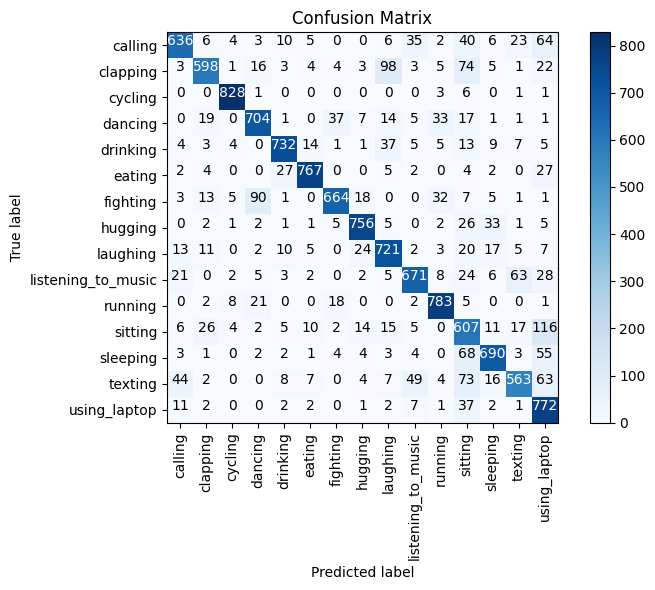
\includegraphics[width=0.5\textwidth]{./images/conf matrix had.png} % Replace with your image file
    \caption{SligLIP 2 Confusion Matrix for Activity Classification}
    \label{fig:HAD-cm}
\end{figure}

% DO WE WANT THIS TO BE SUB- OR SUBSUB SECTION ????????????????????????????
\subsubsection{Finetuning}
Because the pre-trained model was not directly trained for the task of medication 
we needed to finetune the model. In order to do so, we manually annotated individual 
frames of the videos in our training set. We annotated a total of X frames, of which
Y were cases where the subject was taking their medicaiton, and Z were cases where
the subject was not taking their medication. This resulted ina class imbalance of 
XY\% which we found to suffice for the task of finetuning. 

% NOT SURE IF WE SPLIT DATA INTO TEST AND TRAIN, IF WE DID REPORT SPLIT HERE?
The task of finetuning improved the model's test performance on the task of medication intake from
an F1 score of 0.53 to 0.75, suggesting a succesful finetuning process. 




\subsection{Working with Videos}
Because the fine-tuned model was trained to classify individual frames, rather than
entire videos, we needed to find a way to efficiently process videos recorded by the
devices. In order to do so, we extracted a total of 10 frames, evenly spaced out over the
entire length of any video. By the application of this approach, we were able to 
process any video while only processing a small fraction of the frames. 
This way we were able to process the entire video, while onlyprocessing a small 
fraction of the frames. Assuming that in at least one of these frames the subject 
would be taking their medication, for the videos that were annotated as such, 
this limited amount of frames is desirable since it hugely drives back computational costs. 


\section{Results}
\begin{figure}[H]
    \centering
    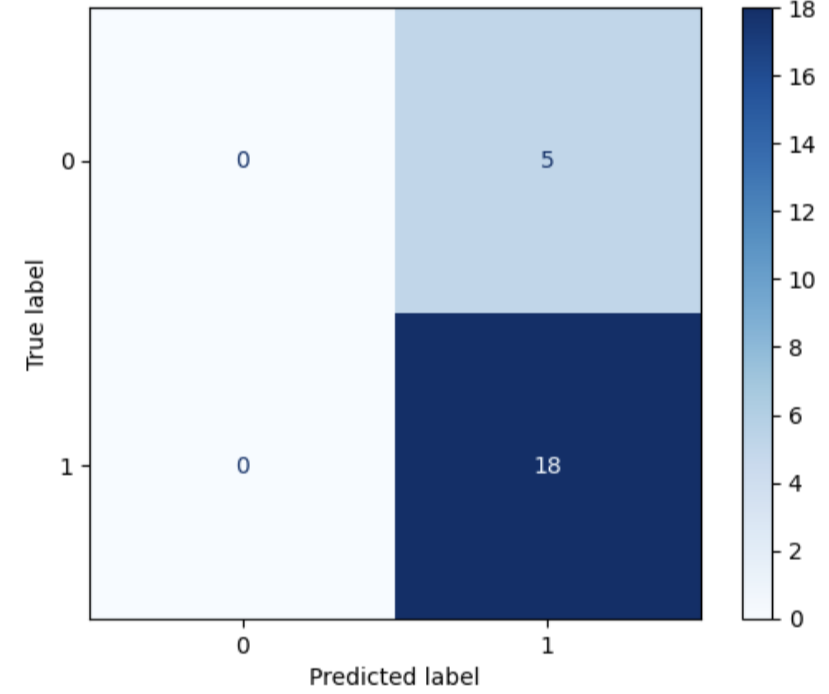
\includegraphics[width=0.5\textwidth]{./images/test confusion matrix.png} % Replace with your image file
    \caption{SligLIP 2 Confusion Matrix for Activity Classification}
    \label{fig:test-cm}
\end{figure}


\section{Conclusion}

\section{Discussion and Recommendations}
\subsection{Data Suggestions}

\section*{References}

\end{document}
